% !TeX root = documentation.tex
% !TeX spellcheck = de_DE

\section{Hintergründe}\label{backgroundinfo}
Um die verschiedenen Eigenschaften anhand vom Lorenz-Modell erklären zu können, sind einige Hintergrundinformationen relevant. Diese davon sind im Folgenden beschrieben.

\subsection{Empfindlichkeit der Anfangsbedingungen}
Unter empfindlichen Anfangsbedingungen versteht man, dass sehr kleine Unterschiede in den Anfangsbedingungen sehr grosse Unterschiede in der Lösungsmenge produzieren. Man nennt dies \textit{sensitive Abhängikeit} und das ist die wesentliche Komponente in chaotischen Systemen. 

So könnte zum Beispiel eine minimale Änderung am Startwert der Lorenz-Gleichungen die Lösung dazu bewirken, dass sie mit gleichbleibenden Parameter gerade auf der gegenüberliegenden Seite des Flügels im Plot zu liegen kommt. In Abbildung \ref{fig:lorenz-startwerte} links ist der Endpunkt gerade sehr nahe am Anfangspunkt (0.9 für $ x, y, z $ ), wobei der Endpunkt in Abbildung \ref{fig:lorenz-startwerte} rechts auf dem anderen Flügel zu liegen kommt. Er ist durch die vielen anderen Werte überdeckt und deshalb nicht sichtbar. Genau das ist also eine Situation wo sich der Endpunkt der rechten Lösung auf dem anderen Flügel befindet als derjenige der linken Lösung. Die einzige Änderung zwischen den zwei Plots ist der Startwert.

\begin{figure}
	\begin{center}$
		\begin{array}{cc}
			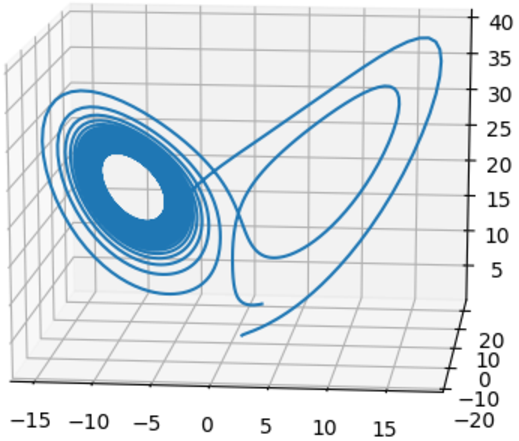
\includegraphics[width=0.5\linewidth]{lorenz/assets/lorenz-modell/lorenz09} &
			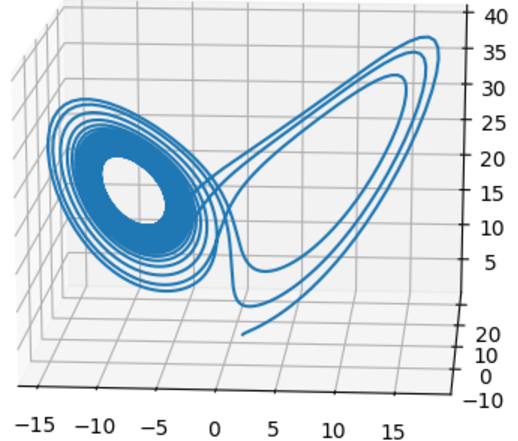
\includegraphics[width=0.5\linewidth]{lorenz/assets/lorenz-modell/lorenz10}
		\end{array}$
		\caption{Bahn des Lorenz-Modell mit Startwert $ x = y = z = 0.9 $ links und $ 1 $ rechts}
		\label{fig:lorenz-startwerte}
	\end{center}
\end{figure}


Es gibt aber auch andere äussere Einwirkungen, die eine Veränderung der Werte auslösen können. Zum Beispiel kann der Rundungsfehler eines CPUs die Ergebnisse klein wenig von Punkt zu Punkt verändern und so werden sich die Fehler kumulieren. Dies führt dazu, dass die Ergebnisse nicht reproduzierbar sind, da solche Einflüsse zwischen Durchläufen variieren.

\subsection{Chaostheorie}
Im Allgemeinen ist die Chaostheorie ein Bereich der Mathematik der sich mit nicht-linearen dynamischen Systemen auseinandersetzt. Wie schon im vorherigen Abschnitt erwähnt ist die wesentliche Komponente eines chaotischen Systems die sensitive Abhängigkeit der Anfangsbedingungen. Sind beliebig kleine Unterschiede darin vorhanden, dann entwickelt sich das System nach einer endlichen Zeit völlig anders. Um das Verhalten eines chaotischen Systems zu einem bestimmten Zeitpunkt zu bestimmen, müssten für die Berechnung unendlich genaue Werte verwendet werden, was praktisch nicht möglich ist. Auch wenn chaotische Systeme deterministisch sind, ist es praktisch oftmals nicht möglich die Resultate an einem gesuchten Zeitpunkt genau zu bestimmen. 


Ein typisches Beispiel für ein chaotisches System ist das Wetter, wie Edward Lorenz herausgefunden hat. Die Modelle von Lorenz sind chaotisch. Dennoch haben diese Systeme aber	 wiederkehrende Verhaltensweisen. Dies zeigt sich, indem sich wiederholende, zum Teil fraktale Muster und ähnliche Figuren zustande kommen. Dadurch, dass die Parameter des Lorenz Modells mit heutiger Technik nicht unendlich genau gemessen werden kann, kann auch keine langfristige und verlässliche Aussage über das Wetter gemacht werden. 

\subsection{Attraktor}
In dynamischen Systemen ist ein Attraktor eine Untermenge eines Phasenraums (Raum aller Zustände), zu welchen sich ein dynamisches System im Laufe der Zeit zubewegt und diese Menge das System nicht mehr verlässt \cite{wikiattraktor}. 
Egal welche Startwerte man in einem Attraktor verwendet, das System entwickelt sich immer auf dieselbe Art und Weise. Beim Lorenz-Attraktor ist dies die berühmte Form des Butterflys. 

Als einfacheres Beispiel für einen Attraktor könnte man ein Pendel nehmen. Ein Pendel entwickelt sich mit der Zeit wegen dem Luftwiderstand und der Reibung immer näher an einen Punkt, bei welchem sich alle darauf wirkenden Kräfte zu 0 addieren und sich das Pendel nicht mehr bewegt. Dieser Punkt ist also der Attraktor für dieses Pendelsystem. Im Unterschied zum Lorenz-Attraktor handelt es sich beim Pendelsystem aber um ein nicht-chaotisches System. Eine kleine Änderung in der Startposition der Masse am Ende des Pendels führt auf eine kleine Änderung in der Position, wobei es bei einem chaotischen System anders ausehen würde. 

Für eine formale Definition eines Attraktors müssen wir also zwei wesentliche Eigenschaften abbilden. Zum Einen muss die Eigenschaft, die Punkte innerhalb einer Toleranz erscheinen lässt, abgebildet werden. Das heisst, dass es zu einem Punkt $P$ des Attraktors  und einer Toleranz $\varepsilon$ eine Zeit $t$ gibt, so dass 

\begin{center}
	$|P - x(t)| < \varepsilon$
\end{center}
wird. Die Bahn geht also zu irgendeinem Zeitpunkt näher als $\varepsilon$ an P vorbei.

Zum Anderen müssen wir die sich wiederholende Komponente definieren. Wir können also beliebig lange warten, es wird immer wieder einen Zeitpunkt geben, zu welcher die Bahn $x(t)$ nahe an P vorbeigeht. Es gibt eine Wartezeit $T$, zu welcher es ein späterer Zeitpunkt $t > T$ gibt, dass
\begin{center}
	$|P - x(t) |< \varepsilon$
\end{center}
gilt.

Die komplette, formale Definition ist also:

\begin{center}\label{Attraktor}
$\forall P, \forall T \text{ und } \forall \varepsilon \text{ } \exists t > T , \text{ für die gilt } |P - x(t) |< \varepsilon$
\end{center}

Für jeden Zeitpunkt $T$ existiert ein späterer Zeitpunkt $t$, bei dem sich die Funktion $x$ (Lorenz-Attraktor) so entwickelt, dass der Betrag der Differenz kleiner als die Toleranz $\varepsilon$ wird. 


\subsection{Strange Attraktor}
Beim Strange Attraktor gilt dieselbe Definition wie für den Attraktor. Das System hat jetzt aber ein viel komplexerer Attraktor als bei einem Pendel. Die Menge des Attraktors besteht nun nicht mehr aus nur einem Punkt, sondern aus einer kompliziert geformten Menge. Das heisst, dass sich Werte innerhalb des Systems chaotisch verhalten. So könnten sich Lösungen in der Definition des Attraktors innerhalb von $\varepsilon$ beliebig bewegen. 